\documentclass[conference]{IEEEtran}
\IEEEoverridecommandlockouts
\usepackage{cite}
\usepackage{amsmath,amssymb,amsfonts}
\usepackage{algorithmic}
\usepackage{graphicx}
\usepackage{textcomp}
\usepackage{xcolor}
\usepackage{booktabs}
\usepackage{multirow}
\usepackage{url}
\usepackage{tikz}
\usetikzlibrary{positioning,arrows.meta,fit}

\newcommand{\evi}{\textsc{EviTrust}}
\newcommand{\eviU}{\textsc{EviTrust}-U}
\newcommand{\eviV}{\textsc{EviTrust}-V}
\newcommand{\todo}[1]{\textcolor{red}{[TODO: #1]}}

\begin{document}

\title{Beyond Popularity: Evidence-Based Trust Prediction\\under Hard-Negative Evaluation}

\author{\IEEEauthorblockN{Anonymous Author(s)}
\IEEEauthorblockA{\textit{Affiliation withheld for review}}}

\maketitle

\begin{abstract}
Trust prediction on social and review platforms is dominated by heterogeneous graph neural networks; the most recent, CAT, reports 0.94 average precision (AP) on Epinions. We show that a single statistic, the product of the trustor's out-degree and the trustee's in-degree, reproduces this number, and that CAT, Guardian, and TrustGuard fall to near chance once test negatives are matched in degree or drawn from the trustor's two-hop neighbourhood. We propose \evi{}, which scores pairs with leakage-safe evidence features (directed paths, activity momentum, and review-order behaviour) kept in an incrementally maintained state, at 2--8\,$\mu$s per record up to a million users, and learned with gradient-boosted trees. Its two pre-registered operating points differ only in their training negatives: \eviU{} uses CAT's uniform negatives, and \eviV{} mixes in hard negatives at a ratio selected on validation data. Against five baselines on Epinions, CiaoDVD, and Wikipedia Requests-for-Adminship, \eviU{} is the best method under the standard protocol on every dataset (Epinions AP 0.970 and MRR 0.759 vs.\ 0.938 and 0.588 for CAT). \eviV{} is the most robust on Epinions and CiaoDVD hard negatives ($+0.20$ to $+0.31$ AP over CAT), also against CAT and TGN re-trained with the same negatives. On wiki-RfA, where most test users are new, CAT falls below chance (AUC 0.42) while \evi{} reaches 0.92--0.94. Robustness transfers only partly to negative families \evi{} was not trained on, and no method separates real oppose votes from support votes much beyond chance.
\end{abstract}

\begin{IEEEkeywords}
trust prediction, link prediction, evaluation protocol, hard negatives, incremental maintenance, gradient boosting
\end{IEEEkeywords}

%=====================================================================
\section{Introduction}
%=====================================================================

Explicit trust links, such as ``I trust this reviewer'' on Epinions or a support vote in a Wikipedia administrator election, drive recommendation, review ranking, and fraud defence on many platforms~\cite{tang2015trust,guha2004propagation}. Predicting which trust links will form next is accordingly a well-studied problem. The field has moved from matrix factorization and propagation models~\cite{yao2013matri,liu2019neuralwalk} through graph convolutional trust evaluators~\cite{lin2020guardian,wang2024trustguard,huo2023trustgnn,jiang2023gatrust} to heterogeneous, time-aware, context-aware graph neural networks. The most recent of these, CAT~\cite{wang2025cat}, combines a user--item heterogeneous graph, continuous-time encodings, and an item-category context layer. It reports an AP of 0.9407 and an AUC of 0.9688 on Epinions, the de facto benchmark of this line of work.

These numbers come from a specific protocol: a chronological split of the trust edges, test negatives drawn uniformly at random at a 1:1 ratio, and metrics computed on test pairs whose endpoints were seen in training. Uniformly random user pairs are almost always pairs of inactive users. A model can separate them from real trust links by asking whether the trustee is popular, without learning anything about trust. Similar concerns have been raised for generic and temporal link prediction~\cite{li2023evaluating,poursafaei2022towards,huang2023tgb}, but not, to our knowledge, for trust prediction.

\textbf{What the benchmark measures.} We first audit the CAT protocol on Epinions (Section~\ref{sec:motivation}). The preferential-attachment score $d^{\text{out}}(u)\cdot d^{\text{in}}(v)$, which uses neither training nor trust semantics, reaches AP 0.941 under the CAT protocol, matching CAT's reported number. We then re-train the original CAT code and score it on two harder negative sets. (b) \emph{Degree-matched} negatives take the trustee from the same in-degree decile as the true trustee. (c) \emph{Two-hop, time-consistent} negatives take a two-hop neighbour of the trustor that already existed when the true link was formed. CAT drops to AP 0.579 and 0.439, against chance levels of 0.453 and 0.399, and its scores correlate with log preferential attachment at Spearman $\rho=0.67$.

\textbf{Evidence instead of popularity.} If popularity explains the benchmark, the remaining question is what \emph{does} predict who trusts whom among users who are equally popular and equally close. Our answer is \emph{evidence available before the trust is formed}:
\begin{itemize}
\item \emph{Directed paths and co-trust}: does $u$ already trust people who trust $v$? Do $u$ and $v$ trust, or are trusted by, the same people?
\item \emph{Activity recency}: is $v$ being trusted by others right now? Has $u$ just started trusting people?
\item \emph{Behavioural evidence from reviews}: have $u$ and $v$ reviewed the same items, did $v$ review them \emph{first}, and do their ratings agree?
\end{itemize}
These signals are cheap, defined for every pair at any time (including new users), and maintainable incrementally as records arrive.

\textbf{Contributions.}
\begin{enumerate}
\item \emph{An evaluation finding.} On the standard Epinions trust benchmark, a degree product reproduces the state-of-the-art AP. Under degree-matched and two-hop time-consistent negatives, CAT, Guardian, and TrustGuard fall to near chance (Sections~\ref{sec:motivation} and~\ref{sec:rq2}).
\item \emph{A method.} \evi{} is a leakage-safe, evidence-based trust predictor. It computes 37 pair features from an incrementally maintained platform state, trains on temporal label windows, and offers two pre-registered operating points that differ only in their training negatives: \eviU{} (CAT's uniform negatives) and \eviV{} (a mixture of uniform and hard negatives, with the ratio selected on validation data). Updates cost 2--8\,$\mu$s per record up to $10^6$ users (Section~\ref{sec:method}).
\item \emph{An evaluation across three platforms, four negative regimes, and five baselines}, including the \emph{real} oppose votes of wiki-RfA as negatives, with paired bootstrap tests on identical test pairs. \eviU{} is the best method under the standard protocol on every dataset. \eviV{} is the most robust on Epinions and CiaoDVD hard negatives, also against CAT and TGN re-trained with the same negatives and on held-out and unseen negative generators. We also report where \evi{} is \emph{not} best: co-review negatives on Epinions, the hard regimes of wiki-RfA, and real distrust, which no method solves (Section~\ref{sec:eval}).
\end{enumerate}

%=====================================================================
\section{Related Work}
\label{sec:related}
%=====================================================================

\textbf{Trust prediction.} Early work inferred trust by factorizing the trust matrix with multi-aspect and transitivity constraints (MATRI~\cite{yao2013matri}), or by propagating trust and distrust along paths~\cite{guha2004propagation}. Content-based models exploit review text and homophily (DeepTrust~\cite{wang2019deeptrust}, C-DeepTrust~\cite{wang2023cdeeptrust}, S-DeepTrust~\cite{wang2023sdeeptrust}). Graph neural trust evaluators learn from the trust graph itself. Guardian~\cite{lin2020guardian} aggregates trustor and trustee roles separately. Medley~\cite{lin2021medley} and DTrust~\cite{wen2023dtrust} add time. TrustGNN~\cite{huo2023trustgnn} learns propagative and composable trust chains. GATrust~\cite{jiang2023gatrust} uses multi-aspect attention. TrustGuard~\cite{wang2024trustguard} adds robustness and explainability. KGTrust~\cite{yu2023kgtrust} and metapath-guided models~\cite{xu2023metapath} incorporate heterogeneous side information. DGTEN~\cite{usman2025dgten} represents nodes and edges as Gaussians for uncertainty-aware dynamic trust evaluation on Bitcoin networks, and TCHG~\cite{liao2026tchg} conditions heterogeneous message passing on three trust-evidence channels with separate temporal states and calibrated probabilities. Both are evaluated with randomly sampled negatives, and our protocol applies to them unchanged. CAT~\cite{wang2025cat} is the most widely compared of these models. It embeds users and items with metapath2vec~\cite{dong2017metapath2vec}, runs heterogeneous attention with continuous-time edge encodings, and mixes per-category predictions through a learned gate. A recent survey~\cite{luo2025gnntrust} lists accuracy on Epinions, Ciao, and Bitcoin under 1:1 random negatives as the standard criterion. We keep CAT's split and data, and change what the negatives are.

\textbf{Link prediction heuristics and learned features.} Neighbourhood heuristics such as common neighbours, Adamic--Adar, Jaccard, and preferential attachment are classic link predictors~\cite{libennowell2007link,adamic2003friends}. Signed-network studies showed that local structural features predict positive and negative links well~\cite{leskovec2010predicting}. Signed GNNs such as SGCN~\cite{derr2018sgcn} and SiGAT~\cite{huang2019sigat} learn from positive and negative links jointly through balance and status theory. Our real-distrust regime (d) is the evaluation counterpart of that line of work: it asks whether a model trained on trust separates trust from distrust. \evi{} belongs to this feature-based tradition. Its features are directed and role-specific, time-indexed, and enriched with review-level behavioural evidence, and the model is learned with gradient-boosted trees~\cite{ke2017lightgbm}.

\textbf{Temporal graph learning.} TGN~\cite{rossi2020tgn}, TGAT~\cite{xu2020tgat}, DySAT~\cite{sankar2020dysat}, and CAW~\cite{wang2021caw} learn node or walk representations on continuous-time graphs. DyGLib~\cite{yu2023dyglib} unifies their implementations. These models are role-agnostic and context-free, which the trust literature cites as the reason for trust-specific architectures~\cite{wang2025cat}.

\textbf{Evaluation of link prediction.} Random negative sampling is known to inflate link prediction results. Li et al.~\cite{li2023evaluating} propose personalised hard negatives (HeaRT) for static link prediction. Poursafaei et al.~\cite{poursafaei2022towards} show that random negatives make memorization baselines competitive in dynamic link prediction and introduce historical and inductive negatives. TGB~\cite{huang2023tgb} standardises these practices for temporal graphs. The popularity shortcut we document is also the evaluation-side twin of popularity bias in recommendation~\cite{abdollahpouri2017popularity}. Our degree-matched and two-hop time-consistent negatives follow the same spirit as these works, adapted to directed trust: they hold popularity and proximity fixed in turn. We are not aware of a prior audit of the trust prediction benchmark, nor of an evaluation that uses real distrust (oppose votes) as negatives.

%=====================================================================
\section{Proposed Method: \evi{}}
\label{sec:method}
%=====================================================================

We first analyse what the standard trust benchmark rewards (Section~\ref{sec:motivation}), since this analysis motivates every design choice of \evi{}, and then present the method.

\subsection{Motivation: What Does the Trust Benchmark Measure?}
\label{sec:motivation}

\textbf{Protocol.} We use CAT's released Epinions data and code~\cite{wang2025cat}: 311{,}158 timestamped trust records (252{,}539 distinct directed pairs) among 9{,}164 users, and 265{,}189 reviews of 12{,}573 items in 25 categories. Trust edges are split chronologically at the 70th and 85th timestamp percentiles into 217{,}837 / 46{,}677 / 46{,}644 train / validation / test records. CAT evaluates on \emph{observed} test pairs, whose endpoints both appear in training (18{,}797 positives), against an equal number of uniformly sampled non-edges.

\textbf{A degree product matches the state of the art.} Table~\ref{tab:motivation} scores this test set with untrained heuristics. Preferential attachment alone reaches AP 0.941 and AUC 0.971, matching CAT's reported 0.9407 / 0.9688. Common neighbours and Adamic--Adar are close behind. Reciprocity carries almost no signal (AP 0.406): 99.98\% of Epinions trust records have a reverse record with an identical timestamp, so both directions always fall in the same split.

\textbf{Hard negatives.} We construct two additional negative sets for the same positives, with a fixed seed shared by all methods.
(b) \emph{Degree-matched}: the negative trustee is drawn from the same in-degree decile (computed on train+validation) as the true trustee.
(c) \emph{Two-hop, time-consistent}: the negative trustee is a two-hop neighbour of the trustor that had already appeared when the positive link was formed; 20\% fall back to (b).
Both sets exclude every observed trust pair. Every heuristic drops to within 0.17 AP of chance. We also re-trained the original CAT code (three seeds, best-validation checkpoint) and scored it on the same pairs. CAT's AP drops from 0.938 to 0.579 on (b) and 0.439 on (c). The headline protocol thus mostly measures whether the trustee is popular, and once popularity and proximity are held fixed a state-of-the-art model is close to chance.

\begin{table}[t]
\centering
\caption{Epinions, observed test pairs. AP under uniform 1:1 negatives (a) and under hard negatives (b, c). CAT is the original code re-trained here (mean of 3 seeds). Heuristics are scored on the E3 uniform negatives, CAT on its own.}
\label{tab:motivation}
\setlength{\tabcolsep}{4pt}
\begin{tabular}{lccc}
\toprule
Scorer & (a) uniform & (b) degree-matched & (c) 2-hop+time \\
\midrule
Chance (prevalence) & 0.346 & 0.453 & 0.399 \\
Reciprocity & 0.406 & -- & -- \\
Preferential attachment & 0.941 & 0.538 & 0.401 \\
Common neighbours & 0.910 & 0.604 & 0.422 \\
Jaccard & 0.875 & 0.620 & -- \\
\midrule
CAT (reported~\cite{wang2025cat}) & 0.9407 & -- & -- \\
CAT (re-trained) & 0.9377 & 0.5790 & 0.4393 \\
\bottomrule
\end{tabular}
\end{table}


\begin{figure*}[t]
\centering
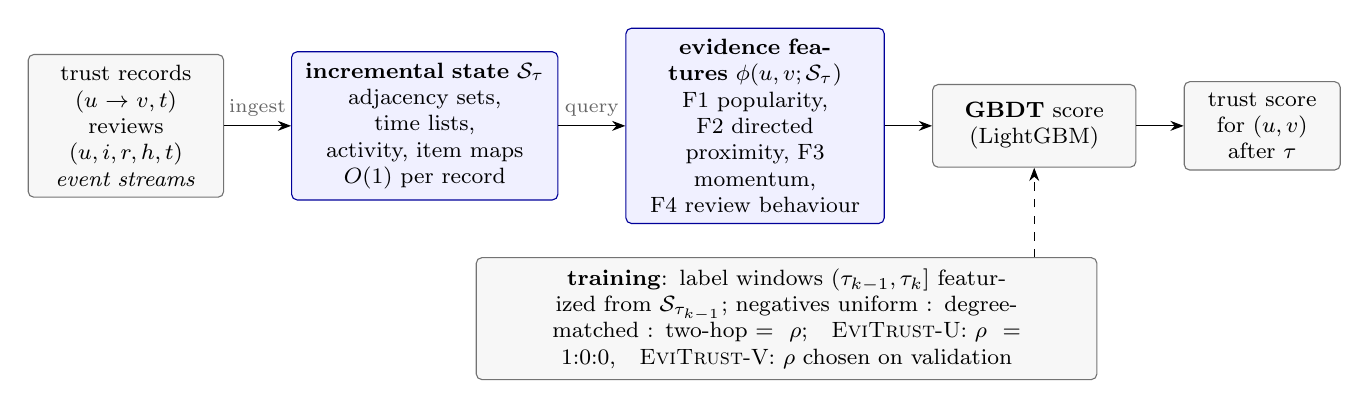
\begin{tikzpicture}[font=\footnotesize, >=Stealth,
  box/.style={draw=black!55, rounded corners=2pt, align=center, inner sep=4pt, minimum height=1.05cm, fill=black!3},
  acc/.style={draw=blue!60!black, rounded corners=2pt, align=center, inner sep=4pt, minimum height=1.05cm, fill=blue!6},
  lab/.style={font=\scriptsize, text=black!60}]
\node[box, text width=2.2cm] (s) {trust records $(u\!\to\!v,t)$\\ reviews $(u,i,r,h,t)$\\ \textit{event streams}};
\node[acc, text width=3.1cm, right=0.85cm of s] (st) {\textbf{incremental state} $\mathcal{S}_\tau$\\ adjacency sets, time lists,\\ activity, item maps\\ $O(1)$ per record};
\node[acc, text width=3.0cm, right=0.85cm of st] (f) {\textbf{evidence features} $\phi(u,v;\mathcal{S}_\tau)$\\ F1 popularity, F2 directed\\ proximity, F3 momentum,\\ F4 review behaviour};
\node[box, text width=2.3cm, right=0.6cm of f] (g) {\textbf{GBDT} score\\ (LightGBM)};
\node[box, text width=1.7cm, right=0.6cm of g] (o) {trust score\\ for $(u,v)$\\ after $\tau$};
\draw[->] (s) -- node[lab, above]{ingest} (st);
\draw[->] (st) -- node[lab, above]{query} (f);
\draw[->] (f) -- (g);
\draw[->] (g) -- (o);
\node[box, text width=7.6cm, below=0.42cm of f.south west, anchor=north west, xshift=-1.9cm, minimum height=0.8cm] (tr)
  {\textbf{training}: label windows $(\tau_{k-1},\tau_k]$ featurized from $\mathcal{S}_{\tau_{k-1}}$; negatives uniform : degree-matched : two-hop $=\rho$;\quad \eviU{}: $\rho=1{:}0{:}0$,\quad \eviV{}: $\rho$ chosen on validation};
\draw[->, dashed] (tr.north -| g.south) -- (g.south);
\end{tikzpicture}
\caption{\evi{} pipeline. Records update a per-user state in $O(1)$; a pair is scored from 37 evidence features computed on demand from the state at prediction time $\tau$. The two operating points differ only in the training negatives.}
\label{fig:pipeline}
\end{figure*}

\subsection{Problem Setting}

Let $U$ be a set of users and $I$ a set of items with categories $c(i)\in C$. The platform produces two timestamped streams: trust records $(u\to v, t)$ and interactions $(u, i, r, h, t)$, where $r$ is a rating and $h$ a helpfulness score. For a time $\tau$, the \emph{platform state} $\mathcal{S}_\tau$ consists of the trust graph $G_\tau=(U,E_\tau)$ with $E_\tau=\{(u,v): (u\to v,t), t\le\tau\}$, together with all interactions with $t<\tau$. Given $\mathcal{S}_\tau$ and a candidate pair $(u,v)\notin E_\tau$, the task is to score how likely $u$ is to trust $v$ after $\tau$. A scorer is \emph{leakage-safe} if the score depends on $\mathcal{S}_\tau$ only. CAT's own test graph (trust up to the test boundary, interactions before it) is exactly $\mathcal{S}_{\tau_{\text{test}}}$.

\subsection{Evidence Features}

\evi{} maps a pair to a vector $\phi(u,v;\mathcal{S}_\tau)\in\mathbb{R}^{37}$ in four families. Let $A$ be the adjacency matrix of $G_\tau$, and let $\mathcal{N}^{+}(u)$ and $\mathcal{N}^{-}(u)$ be the out- and in-neighbours of $u$, and $\mathcal{N}(u)$ their union.

\textbf{(F1) Popularity and activity volume} (5 features): $\log(1+\cdot)$ of the out- and in-degrees of $u$ and $v$, and the preferential attachment $\log(1+d^{+}(u)d^{-}(v))$. These let the model use popularity when it is informative. They are not its only signal.

\textbf{(F2) Directed proximity} (14 features): reciprocity $A_{vu}$; directed path counts $(A^2)_{uv}=|\mathcal{N}^{+}(u)\cap\mathcal{N}^{-}(v)|$ and $(A^3)_{uv}$, normalized by $d^{+}(u)$, $d^{-}(v)$, and $d^{+}(u)d^{-}(v)$; common trustees $|\mathcal{N}^{+}(u)\cap\mathcal{N}^{+}(v)|$ and common trustors $|\mathcal{N}^{-}(u)\cap\mathcal{N}^{-}(v)|$ with cosine normalization; and undirected common neighbours, Adamic--Adar, resource allocation, and Jaccard. Unlike symmetric heuristics, the directed counts separate ``$u$ trusts people who trust $v$'' from ``$u$ and $v$ are trusted by the same people''.

\textbf{(F3) Temporal activity} (7 features): days since the last activity of $u$ and of $v$ (any trust record or interaction before $\tau$); account age of $u$ and $v$; the number of trust links $v$ received and $u$ issued in the last 180 days; and the fraction of $v$'s in-links that are recent. These capture the \emph{momentum} of trust: who is being trusted right now, and who is actively trusting.

\textbf{(F4) Behavioural evidence} (11 features): review counts of $u$ and $v$; the number of co-reviewed items, also normalized by $\sqrt{n_u n_v}$; the \emph{reading-order} counts $|\{i: t_{v,i} < t_{u,i}\}|$ and $|\{i: t_{u,i} < t_{v,i}\}|$, i.e., how often $v$ reviewed a shared item before $u$ (a proxy for $u$ having read $v$'s review); the mean absolute rating difference on co-reviewed items; the cosine similarity of the two users' category profiles; and the mean rating of $u$ and of $v$ and the mean helpfulness of $v$.

Optionally, (F5) adds the dot product and cosine of the users' metapath2vec embeddings~\cite{dong2017metapath2vec} (the embeddings CAT consumes). Section~\ref{sec:ablation} shows that \evi{} does not need them, and our streaming implementation omits them.

\subsection{Incremental State and Query}
\label{sec:stream}

\evi{} never materializes a graph representation that must be re-learned. Its state $\mathcal{S}_\tau$ (Fig.~\ref{fig:pipeline}) is the following set of per-user structures, each updated in $O(1)$ when a record arrives:
directed and undirected adjacency sets $\mathcal{N}^{+},\mathcal{N}^{-},\mathcal{N}$;
an append-only, time-sorted list of each user's incoming and outgoing trust times;
first and last activity times;
review count, rating sum, helpfulness sum, and a category histogram;
and a map from each reviewed item to (first review time, rating).
Pair features are evaluated on demand. $(A^2)_{uv}$ is one set intersection. $(A^3)_{uv}=\sum_{x\in\mathcal{N}^{-}(v)}|\mathcal{N}^{+}(u)\cap\mathcal{N}^{-}(x)|=\sum_{w\in\mathcal{N}^{+}(u)}|\mathcal{N}^{+}(w)\cap\mathcal{N}^{-}(v)|$ is evaluated over the smaller of $\mathcal{N}^{+}(u)$ and $\mathcal{N}^{-}(v)$. Common-neighbour scores intersect the undirected sets. The 180-day counts use binary search on the time lists, and the co-review statistics intersect the two item maps.
State size is $O(|U|+|E|+|\text{interactions}|)$. On all three datasets the streaming features equal those of a dense matrix implementation up to float32 rounding (maximum relative difference $1.6\times10^{-7}$ over 5{,}000 pairs per dataset), so every accuracy result below holds for the streaming system.

\subsection{Leakage-Safe Training on Temporal Label Windows}

Training a pair classifier on edges that are already in the graph used for its features leaks the label into the features, because a training edge contributes to its own path counts. \evi{} instead builds its training set from \emph{label windows} inside the training period. For boundaries $\tau_0<\tau_1<\tau_2$ (the 50th, 60th, and 70th percentiles of trust timestamps; $\tau_2$ is CAT's validation boundary), the positives of window $k$ are the distinct pairs that first appear in $(\tau_{k-1},\tau_k]$, featurized from $\mathcal{S}_{\tau_{k-1}}$. Validation pairs (CAT's validation edges) are featurized from $\mathcal{S}_{\tau_{\text{val}}}$, and test pairs from $\mathcal{S}_{\tau_{\text{test}}}$. Training, model selection, and testing thus all mimic deployment: score pairs \emph{now}, observe links \emph{later}.

\subsection{Training Negatives and the Two Operating Points}

For every positive $(u,v,t)$ in a label window, \evi{} draws negatives from three generators against the window-start state: uniform (as in CAT), degree-matched (same in-degree decile as $v$), and two-hop time-consistent (a two-hop neighbour of $u$ that existed at $t$). The ratio $\rho=(\rho_{\text{uni}}:\rho_{\text{deg}}:\rho_{\text{2hop}})$ of negatives per positive sets the operating point. Both operating points below were fixed in a pre-registration before their test results were computed.
\begin{itemize}
\item \eviU{}, $\rho=(1{:}0{:}0)$: CAT's own uniform 1:1 regime. This is the like-for-like comparison on the standard protocol.
\item \eviV{}: for each dataset and seed, $\rho$ is chosen among the three ratios 1:0:0, 3:1:1, and 1:1:1 by the mean validation AP over the three validation negative regimes (uniform, degree-matched, two-hop). On all datasets and seeds the rule selected a mixed ratio, (3:1:1) in four cases and (1:1:1) in five, and never the uniform one.
\end{itemize}
Positives are re-weighted to balance the classes.

\subsection{Model and Selection}

We use LightGBM~\cite{ke2017lightgbm} (learning rate 0.03, up to 2{,}000 trees, row and column subsampling 0.8, $L_2=1$, at least 50 samples per leaf). The number of leaves $\in\{31,127\}$ and the number of trees (in steps of 100) are selected on the validation pairs only, by the mean validation AP over the three validation negative regimes. The same criterion selects $\rho$ for \eviV{}. Training on Epinions uses 48{,}410 positive pairs.

%=====================================================================
\section{Performance Evaluation}
\label{sec:eval}
%=====================================================================

\subsection{Setup}

\textbf{Datasets.} Table~\ref{tab:data} summarizes the data.
\emph{Epinions} is CAT's release, used unchanged.
\emph{CiaoDVD}~\cite{guo2014etaf} has directed trust and DVD ratings in 17 genres, but no trust timestamps. A common workaround synthesizes a trust time from the users' last rating date, which leaks future activity into the split. We avoid this by splitting the trust edges uniformly at random (70/15/15) and making every rating visible to every split, i.e., a static link-prediction setting.
\emph{wiki-RfA}~\cite{west2014exploiting} contains 198{,}275 timestamped votes in Wikipedia administrator elections. A support vote $u\to v$ is a trust link with its real time, and the split is CAT's chronological 70/85\% split. Elections act as items: every vote is an interaction, with the vote value as rating. Elections have no categories, so a single category is used. The 35{,}886 \emph{oppose} votes provide real distrust, which we use as an additional negative regime.

\begin{table}[t]
\centering
\caption{Dataset statistics (users and interactions restricted to the trust graph).}
\label{tab:data}
\setlength{\tabcolsep}{3.5pt}
\begin{tabular}{lrrr}
\toprule
& Epinions & CiaoDVD & wiki-RfA \\
\midrule
Users & 9{,}164 & 4{,}658 & 9{,}786 \\
Items (categories) & 12{,}573 (25) & 13{,}067 (17) & 3{,}783 (1) \\
Trust records & 311{,}158 & 40{,}133 & 137{,}911 \\
User--item interactions & 265{,}189 & 34{,}438 & 187{,}415 \\
Split & chronological & random & chronological \\
Test positives (observed) & 46{,}644 (18{,}797) & 6{,}020 (5{,}663) & 20{,}687 (1{,}182) \\
Real negatives & -- & -- & 35{,}886 oppose \\
\bottomrule
\end{tabular}
\end{table}

\textbf{Baselines.} We compare against five baselines that cover the main families of trust and temporal link prediction.
(i) \emph{CAT}~\cite{wang2025cat}: the released code, unchanged, with its default hyper-parameters. On CiaoDVD and wiki-RfA we train dataset-specific metapath2vec ($u$--$i$--$c$--$i$--$u$) embeddings on interactions before the test boundary and size CAT's category gate to the number of categories.
(ii) \emph{Heuristic-LR}: logistic regression on five classic heuristics (reciprocity, preferential attachment, common neighbours, Adamic--Adar, Jaccard), trained exactly like \eviU{} (same label windows, states, and uniform negatives). It isolates the value of \evi{}'s richer evidence and model.
(iii) \emph{Guardian}~\cite{lin2020guardian} and (iv) \emph{TrustGuard}~\cite{wang2024trustguard}: faithful re-implementations of their released layer algebra (Guardian one layer of 64 units; TrustGuard 32--64--32 with four equal-time snapshots and temporal attention) with a link-prediction head. They take the same metapath2vec user features as CAT, are trained full-batch for 200 epochs against uniform 1:1 negatives resampled every epoch, and use the epoch with the best validation AP.
(v) \emph{TGN}~\cite{rossi2020tgn}: PyG's TGN memory (dimension 100) with graph-attention embeddings over the 10 most recent neighbours, trained chronologically with uniform negatives for up to 30 epochs with validation early stopping.
All message-passing models use the training graph during training and validation and the train+validation graph at test time. TGN scores test pairs from its memory at the test boundary, so every method sees the same platform state $\mathcal{S}_{\tau_{\text{test}}}$.

\textbf{Negative regimes.} (a) \emph{CAT protocol}: CAT's own uniform 1:1 test negatives, regenerated with CAT's code and random sequence; (b) degree-matched; (c) two-hop time-consistent; (d) wiki-RfA only: test-period oppose votes that are not trust pairs. All methods score \emph{identical} pairs. Re-scoring our CAT checkpoints reproduces all twelve Epinions AP values of the original runs to four decimals.

\textbf{Metrics and tests.} Following CAT, we report AP, AUC, and MRR (each positive ranked against 100 sampled negatives, ties averaged) on observed pairs, and additionally on all pairs for wiki-RfA. All numbers are means over seeds 42, 43, and 44, recomputed from per-pair score files with the same code for every method. For each seed, we test the AP difference between \evi{} and each baseline with a paired bootstrap over test pairs ($B=1{,}000$). We report the number of seeds whose 95\% interval lies above zero and the number whose interval lies below zero.

\textbf{Research questions.}
RQ1: Does \evi{} improve the headline benchmark?
RQ2: Is it robust to hard negatives, and is that robustness due to its training negatives alone?
RQ3: Does it depend on popularity?
RQ4: Which evidence matters?
RQ5: How does it handle new users and real distrust?
RQ6: What do updates, queries, and scale cost?

\begin{table*}[t]
\centering
\caption{RQ1: CAT protocol (a), observed test pairs, mean over 3 seeds (AP $\pm$ s.d.). Best in bold.}
\label{tab:main}
\setlength{\tabcolsep}{5pt}
\begin{tabular}{l|ccc|ccc|ccc}
\toprule
& \multicolumn{3}{c|}{Epinions} & \multicolumn{3}{c|}{CiaoDVD} & \multicolumn{3}{c}{wiki-RfA} \\
Method & AP & AUC & MRR & AP & AUC & MRR & AP & AUC & MRR \\
\midrule
CAT (reported~\cite{wang2025cat}) & 0.9407 & 0.9688 & 0.6758 & -- & -- & -- & -- & -- & -- \\
CAT (re-trained) & 0.9377$\pm$.003 & 0.9685 & 0.5882 & 0.9440$\pm$.002 & 0.9362 & 0.4706 & 0.4201$\pm$.020 & 0.8009 & 0.2953 \\
Heuristic-LR & 0.9158$\pm$.000 & 0.9126 & 0.6445 & 0.9829$\pm$.000 & 0.9804 & 0.7154 & 0.4142$\pm$.004 & 0.7511 & 0.2967 \\
Guardian & 0.8713$\pm$.013 & 0.9356 & 0.4044 & 0.9627$\pm$.001 & 0.9689 & 0.4980 & 0.3223$\pm$.010 & 0.7594 & 0.2245 \\
TrustGuard & 0.9254$\pm$.008 & 0.9640 & 0.5586 & 0.9554$\pm$.008 & 0.9644 & 0.4578 & 0.5162$\pm$.039 & 0.8873 & 0.3421 \\
TGN & 0.8594$\pm$.003 & 0.9039 & 0.4489 & 0.9287$\pm$.005 & 0.9171 & 0.4152 & 0.2981$\pm$.034 & 0.7790 & 0.1896 \\
\midrule
\eviU{} & \textbf{0.9703}$\pm$.001 & \textbf{0.9833} & \textbf{0.7588} & \textbf{0.9866}$\pm$.000 & \textbf{0.9845} & \textbf{0.7512} & \textbf{0.7281}$\pm$.049 & \textbf{0.9080} & \textbf{0.5804} \\
\eviV{} & 0.9384$\pm$.016 & 0.9678 & 0.6057 & 0.9712$\pm$.004 & 0.9673 & 0.6002 & 0.5252$\pm$.099 & 0.8522 & 0.3709 \\
\bottomrule
\end{tabular}
\end{table*}

\subsection{RQ1: The Standard Protocol}

Table~\ref{tab:main} reports the CAT protocol. \eviU{}, trained with the same uniform negatives as CAT, is the best method on all three datasets in AP, AUC, and MRR. It is significantly above \emph{every} baseline in every seed (15 of 15 comparisons, Table~\ref{tab:paired}). On Epinions it gains $+0.033$ AP, $+0.015$ AUC, and $+0.171$ MRR over CAT, and it also exceeds CAT's reported numbers (0.9407 / 0.9688 / 0.6758). On wiki-RfA it leads the strongest baseline, TrustGuard, by $+0.21$ AP. On CiaoDVD the margin over Heuristic-LR is small ($+0.004$ AP), although still significant; on this random split the five classic heuristics are already a strong predictor (Section~\ref{sec:rq2}).
Two further observations bear on the benchmark question. First, Guardian, TrustGuard, and TGN all score \emph{below} CAT on Epinions, and Heuristic-LR is within 0.022 of it. Second, TGN is the weakest baseline on Epinions (a) but the strongest on hard negatives (Table~\ref{tab:hard}). The uniform protocol thus ranks methods partly by how much they exploit popularity.
\eviV{}, which trades popularity for robustness (RQ3), is on par with CAT on Epinions (a) ($+0.001$; above CAT in 2 seeds, below in 1), above it on CiaoDVD ($+0.027$, 3/3 seeds) and wiki-RfA ($+0.105$, 2/3), and 0.012 below Heuristic-LR on CiaoDVD.

\begin{table}[t]
\centering
\caption{RQ2: AP under hard negatives, observed pairs, mean of 3 seeds. Best in bold.}
\label{tab:hard}
\setlength{\tabcolsep}{2.6pt}
\begin{tabular}{l|cc|cc|ccc}
\toprule
& \multicolumn{2}{c|}{Epinions} & \multicolumn{2}{c|}{CiaoDVD} & \multicolumn{3}{c}{wiki-RfA} \\
Method & (b) & (c) & (b) & (c) & (b) & (c) & (d) \\
\midrule
chance & .453 & .399 & .494 & .487 & .205 & .181 & .760 \\
CAT & .579 & .439 & .543 & .538 & .413 & .136 & .751 \\
Heur.-LR & .562 & .420 & .745 & .737 & .383 & .140 & .778 \\
Guardian & .490 & .406 & .543 & .509 & .371 & .142 & .767 \\
TrustGuard & .561 & .453 & .531 & .503 & \textbf{.523} & .235 & .744 \\
TGN & .742 & .617 & .671 & .566 & .483 & .258 & \textbf{.784} \\
\midrule
\eviU{} & .714 & .541 & .787 & .741 & .457 & .219 & .779 \\
\eviV{} & \textbf{.783} & \textbf{.662} & \textbf{.848} & \textbf{.836} & .444 & \textbf{.352} & .765 \\
\bottomrule
\end{tabular}
\end{table}

\begin{table}[t]
\centering
\caption{Paired bootstrap ($B$=1000), observed pairs: mean AP difference of \evi{} to the \emph{strongest baseline} of each regime (by mean AP), with the number of seeds (of 3) whose 95\% CI is above 0 / below 0.}
\label{tab:paired}
\setlength{\tabcolsep}{2.4pt}
\begin{tabular}{llcc}
\toprule
Dataset & Regime (strongest baseline) & \eviU{} & \eviV{} \\
\midrule
\multirow{3}{*}{Epinions} & (a) (CAT) & +.033 (3/0) & +.001 (2/1) \\
& (b) (TGN) & $-$.028 (0/2) & +.041 (3/0) \\
& (c) (TGN) & $-$.076 (0/3) & +.045 (3/0) \\
\midrule
\multirow{3}{*}{CiaoDVD} & (a) (Heuristic-LR) & +.004 (3/0) & $-$.012 (0/3) \\
& (b) (Heuristic-LR) & +.042 (3/0) & +.102 (3/0) \\
& (c) (Heuristic-LR) & +.004 (1/1) & +.099 (3/0) \\
\midrule
\multirow{4}{*}{wiki-RfA} & (a) (TrustGuard) & +.212 (3/0) & +.009 (1/1) \\
& (b) (TrustGuard) & $-$.066 (0/3) & $-$.079 (0/3) \\
& (c) (TGN) & $-$.039 (0/2) & +.093 (3/0) \\
& (d) (TGN) & $-$.005 (0/0) & $-$.018 (0/0) \\
\bottomrule
\end{tabular}
\end{table}

\subsection{RQ2: Hard Negatives}
\label{sec:rq2}

Table~\ref{tab:hard} keeps the positives fixed and replaces the negatives. On Epinions and CiaoDVD, CAT, Guardian, and TrustGuard collapse to within $0.13$ AP of chance on (b) and (c). Popularity reliance is therefore a property of the trust-GNN family, not of CAT alone. \eviV{} is the most robust method on both datasets. It reaches 0.783 / 0.662 on Epinions and 0.848 / 0.836 on CiaoDVD, i.e., $+0.20$ to $+0.31$ over CAT, and it is significantly above the strongest baseline in every seed (Table~\ref{tab:paired}).

Two baselines are notably stronger than the rest. \emph{TGN}, which learns from the event stream with a node memory, reaches 0.742 / 0.617 on Epinions. That is significantly better than \eviU{} but below \eviV{} ($+0.041$ and $+0.045$, 3/3 seeds). \emph{Heuristic-LR} is strong on CiaoDVD (0.745 / 0.737), because under a random split the reverse edge of a test link is often in the training graph (31.7\% of observed test positives). \eviV{} still improves on it by $+0.10$ on both regimes. Even on the positives whose reverse edge is \emph{not} in the graph, \eviU{} keeps its lead under the CAT protocol (AP 0.967 vs.\ 0.958 for Heuristic-LR and 0.902 for CAT), so \evi{}'s advantage is not reciprocity alone.

On wiki-RfA observed pairs the picture is mixed. TrustGuard is best on degree-matched negatives (0.523), significantly above both \evi{} variants. \eviV{} is best on two-hop negatives (0.352, $+0.093$ over TGN, 3/3). We discuss (d) in RQ5.

\textbf{Control: the same training negatives for the neural models.} The \eviU{}/\eviV{} contrast shows that the training negatives matter. If they were \emph{sufficient}, the neural models should match \eviV{} when trained the same way. We therefore re-train CAT and TGN as \emph{CAT-H} and \emph{TGN-H} with \evi{}'s mixed negatives. Each positive gets one negative (keeping CAT's 1:1 balance), drawn as uniform, degree-matched, or two-hop with probability 3/5, 1/5, 1/5 from the same generators. The selected epoch maximizes the mean validation AP on (b) and (c) among epochs whose validation AP on (a) is within 0.005 of the best, using \evi{}'s validation negatives. The architectures, neighbour sampling, losses, and optimizers are unchanged. These are controls, not published methods, and are therefore kept out of Tables~\ref{tab:main} and~\ref{tab:hard}.
Table~\ref{tab:control} shows that the mixed negatives do not close the gap. CAT-H trades accuracy on (a) for small gains on (b) and (c) on Epinions only. On CiaoDVD its validation AP on (a) peaks after the first epoch in every seed. TGN-H improves TGN on Epinions hard negatives ($+0.019$, $+0.033$) but loses $0.043$ on (a). \eviV{} remains significantly better than both controls in all 12 Epinions and CiaoDVD comparisons (3/3 seeds), including against TGN-H on (b) and (c) ($+0.023$, $+0.012$). On wiki-RfA the mixed negatives lower both neural models on (a) and (b). The one exception is real distrust (d), where TGN-H reaches 0.814 (observed, s.d.\ 0.028). Training negatives are thus necessary for robustness but not sufficient; the evidence features and the model account for the rest.

\textbf{Generalization to unseen hard negatives.} \eviV{} is trained with the degree-matched and two-hop generators that also produce test regimes (b) and (c). We therefore test it on hard negatives it has not seen, in two ways. (i) \emph{Leave one generator out}: V$-$c is trained with $\rho=(3{:}1{:}0)$, selected on validation (a) and (b), and evaluated on (c); V$-$b is trained with $\rho=(3{:}0{:}1)$, selected on validation (a) and (c), and evaluated on (b). (ii) \emph{Unseen generators}, used by no model for training or selection: (e) \emph{co-review} negatives are users who reviewed (voted on) an item that $u$ reviewed, both before $t$; (f) \emph{active degree-matched} negatives come from $v$'s in-degree decile and were active in the 30 days before $t$. Table~\ref{tab:unseen} reports all methods. The neural baselines were re-trained with the same seeds for this run, and their (a)--(c) values differ from Tables~\ref{tab:main} and~\ref{tab:hard} by at most 0.01.
On Epinions and CiaoDVD robustness largely transfers. V$-$b stays above the strongest baseline on the held-out (b) ($+0.022$ over TGN, $+0.038$ over Heuristic-LR, 3/3 seeds). V$-$c beats Heuristic-LR on CiaoDVD (c) ($+0.022$, 3/3) and ties TGN on Epinions (c) ($-0.006$, not significant). \eviV{} leads on (f) ($+0.042$ over TGN and $+0.102$ over Heuristic-LR, 3/3). Holding a generator out still costs 0.02--0.08 AP on its regime, so part of \eviV{}'s margin does come from matching the training negatives.
Co-review negatives are the clearest failure. They share exactly the behavioural evidence that F4 exploits, and on Epinions TGN beats \eviV{} on them by 0.091 AP (3/3). On wiki-RfA TrustGuard is best on (b) and (f), and TrustGuard or TGN is best on the held-out generators, while \evi{} leads only on (c) and, by a point estimate, (e). Robustness to one family of hard negatives does not imply robustness to another, which is why we recommend reporting several families.

\begin{table}[t]
\centering
\caption{Unseen hard negatives (observed AP, mean of 3 seeds): (e) co-review and (f) active degree-matched negatives, used by no model for training or selection. The last two rows hold one generator out of \eviV{}'s training and selection and report the held-out regime. Best in bold.}
\label{tab:unseen}
\setlength{\tabcolsep}{2.2pt}
\begin{tabular}{l|cc|cc|cc}
\toprule
& \multicolumn{2}{c|}{Epinions} & \multicolumn{2}{c|}{CiaoDVD} & \multicolumn{2}{c}{wiki-RfA} \\
Method & (e) & (f) & (e) & (f) & (e) & (f) \\
\midrule
CAT & .595 & .514 & .608 & .540 & .146 & .359 \\
Heur.-LR & .635 & .517 & .761 & .740 & .136 & .344 \\
Guardian & .582 & .504 & .567 & .542 & .171 & .406 \\
TrustGuard & .600 & .489 & .592 & .527 & .270 & \textbf{.496} \\
TGN & \textbf{.772} & .559 & .701 & .665 & .268 & .444 \\
\midrule
\eviU{} & .674 & .567 & \textbf{.779} & .782 & .199 & .351 \\
\eviV{} & .681 & \textbf{.601} & .773 & \textbf{.842} & \textbf{.289} & .391 \\
\midrule
& \multicolumn{6}{c}{held-out regime, AP (strongest baseline)} \\
V$-$c on (c) & \multicolumn{2}{c|}{.610 (TGN .616)} & \multicolumn{2}{c|}{\textbf{.759} (H-LR .737)} & \multicolumn{2}{c}{.240 (TGN .259)} \\
V$-$b on (b) & \multicolumn{2}{c|}{\textbf{.763} (TGN .740)} & \multicolumn{2}{c|}{\textbf{.784} (H-LR .745)} & \multicolumn{2}{c}{.340 (TrustGuard .523)} \\
\bottomrule
\end{tabular}
\end{table}

\begin{table}[t]
\centering
\caption{Control (observed AP, mean of 3 seeds): CAT and TGN re-trained with \evi{}'s mixed negatives (CAT-H, TGN-H). Last two rows: paired bootstrap AP difference of \eviV{}; every difference has its 95\% CI above 0 in all 3 seeds.}
\label{tab:control}
\setlength{\tabcolsep}{3pt}
\begin{tabular}{l|ccc|ccc}
\toprule
& \multicolumn{3}{c|}{Epinions} & \multicolumn{3}{c}{CiaoDVD} \\
Method & (a) & (b) & (c) & (a) & (b) & (c) \\
\midrule
CAT (uniform) & .938 & .579 & .439 & .944 & .543 & .538 \\
CAT-H (mixed) & .894 & .635 & .493 & .881 & .532 & .514 \\
TGN (uniform) & .859 & .742 & .617 & .929 & .671 & .566 \\
TGN-H (mixed) & .816 & .760 & .650 & .914 & .682 & .584 \\
\eviV{} (mixed) & \textbf{.938} & \textbf{.783} & \textbf{.662} & \textbf{.971} & \textbf{.848} & \textbf{.836} \\
\midrule
\eviV{} $-$ CAT-H & +.045 & +.149 & +.169 & +.090 & +.316 & +.322 \\
\eviV{} $-$ TGN-H & +.122 & +.023 & +.012 & +.057 & +.166 & +.252 \\
\bottomrule
\end{tabular}
\end{table}


\begin{figure*}[t]
\centering
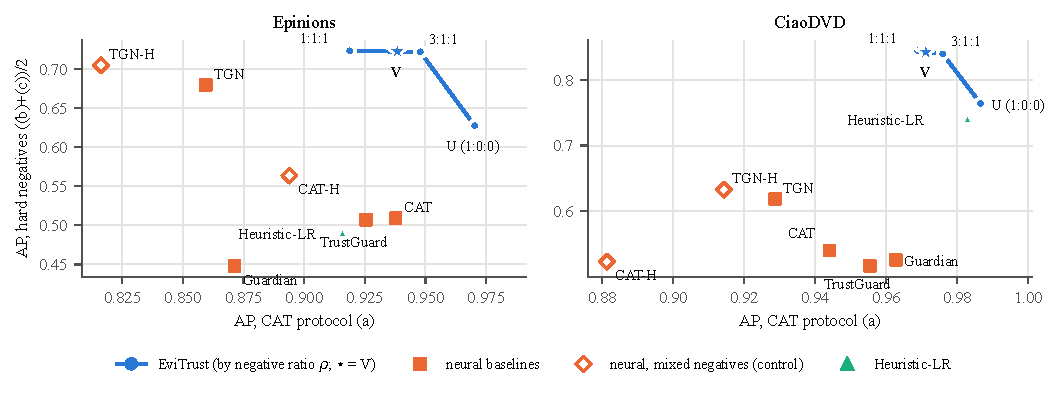
\includegraphics[width=\textwidth]{fig_tradeoff.pdf}
\caption{The popularity--robustness trade-off (observed pairs, mean of 3 seeds). $x$: AP under the CAT protocol (a); $y$: mean AP over the hard negatives (b) and (c). The blue curve shows \evi{} as the training-negative ratio $\rho$ moves from uniform (\eviU{}) to mixed; the star is the validation-selected \eviV{}. Hollow markers are CAT and TGN re-trained with the same mixed negatives (RQ2 control). Every baseline and control is Pareto-dominated by at least one point of the \evi{} curve.}
\label{fig:tradeoff}
\end{figure*}

\subsection{RQ3: Reliance on Popularity}

We correlate each model's Epinions scores on observed test positives with log preferential attachment. \eviU{} is as popularity-correlated as CAT (Spearman $\rho=0.672$ vs.\ $0.670$): both exploit popularity under uniform negatives. \eviU{}, however, also ranks correctly \emph{within} popularity strata, which CAT does not, as their (b) results show (0.714 vs.\ 0.579). \eviV{} reduces the correlation to $\rho=0.291$. The pattern holds on the other datasets: CAT, \eviU{}, and \eviV{} reach $\rho=0.73$, $0.62$, and $0.28$ on CiaoDVD and $0.51$, $0.13$, and $-0.07$ on wiki-RfA. It gives up $0.032$ AP on (a) relative to \eviU{} and gains $0.07$--$0.12$ on (b) and (c). The negative ratio thus exposes an explicit trade-off between the popularity-driven benchmark and hard-negative robustness (Fig.~\ref{fig:tradeoff}), and the pre-registered validation rule places \eviV{} at the robust end of it. In practice, \eviU{} suits reporting on the uniform protocol, while \eviV{} suits deployment, where candidate lists are dominated by active and nearby users. CAT offers no such control. TGN sits at the robust end of the same trade-off (weak on (a), strong on (b, c)) but below \eviV{} on both axes, and on both datasets every baseline and every control is Pareto-dominated (lower on both axes) by at least one \evi{} operating point.

\subsection{RQ4: Which Evidence Matters?}
\label{sec:ablation}

Table~\ref{tab:ablation} removes feature families on Epinions (mean of 3 seeds), for \eviU{} and for the mixed 3:1:1 configuration that \eviV{} selects in two of three Epinions seeds.
(i) The metapath2vec embeddings that CAT relies on are \emph{unnecessary}: removing them changes AP by $-0.002$ to $+0.005$, and \eviU{} without them reaches 0.969 on (a), so \evi{}'s gains do not come from CAT's inputs.
(ii) Behavioural evidence matters most when the model is pushed beyond popularity. Removing F4 costs the mixed configuration 0.028 AP on (a) and 0.015 on (b), and costs the 1:1:1 configuration 0.049 on (a).
(iii) Structure alone (F1--F3, no reviews, no embeddings) still beats CAT by a wide margin on (b) and (c) (0.763 / 0.646 vs.\ 0.579 / 0.439).
(iv) The five classic heuristics alone (Heuristic-LR, Table~\ref{tab:main}) reach only 0.916 / 0.562 / 0.420, so directed, temporal, and behavioural evidence account for most of \evi{}'s advantage on this chronological benchmark.
By LightGBM gain, the most important features of the mixed configuration are temporal: days since $v$'s last activity, the recent fraction of $v$'s in-links, days since $u$'s last activity, and $u$'s recent out-links, followed by $v$'s out-degree, account age, and helpfulness. Trust formation on Epinions is strongly \emph{momentum-driven}. CAT's per-edge time encoding does not capture this, since its scores are dominated by static popularity.

\begin{table}[t]
\centering
\caption{RQ4: ablation on Epinions (observed AP, mean $\pm$ s.d.\ over 3 seeds). The mixed configurations use the selection rule of the development variant described in Section~\ref{sec:threats}.}
\label{tab:ablation}
\setlength{\tabcolsep}{2.4pt}
\begin{tabular}{lccc}
\toprule
Variant & (a) & (b) & (c) \\
\midrule
CAT & 0.938 & 0.579 & 0.439 \\
\midrule
\eviU{} (all features) & 0.970$\pm$.001 & 0.714$\pm$.019 & 0.541$\pm$.023 \\
\quad $-$ embeddings (F5) & 0.969$\pm$.003 & 0.716$\pm$.012 & 0.546$\pm$.013 \\
\quad $-$ behavioural evidence (F4) & 0.967$\pm$.001 & 0.711$\pm$.010 & 0.541$\pm$.014 \\
\midrule
Mixed 3:1:1 (all features) & 0.948$\pm$.000 & 0.784$\pm$.001 & 0.661$\pm$.001 \\
\quad $-$ embeddings (F5) & 0.950$\pm$.002 & 0.782$\pm$.002 & 0.659$\pm$.003 \\
\quad $-$ behavioural evidence (F4) & 0.920$\pm$.001 & 0.769$\pm$.002 & 0.660$\pm$.001 \\
\quad structure only (F1--F3) & 0.919$\pm$.005 & 0.763$\pm$.002 & 0.646$\pm$.002 \\
\midrule
Mixed 1:1:1 (all features) & 0.919$\pm$.001 & 0.782$\pm$.001 & 0.665$\pm$.003 \\
\quad $-$ behavioural evidence (F4) & 0.870$\pm$.002 & 0.766$\pm$.001 & 0.671$\pm$.002 \\
\bottomrule
\end{tabular}
\end{table}

\subsection{RQ5: New Users and Real Distrust (wiki-RfA)}

wiki-RfA is the most realistic of the three settings. The chronological test period (April 2010 onward) is dominated by users who were not active in training: only 1{,}182 of 20{,}687 test positives are observed. Table~\ref{tab:rfa} reports all test pairs. CAT's AUC is 0.415 and Guardian's 0.498, \emph{at or below chance}, while \evi{} reaches 0.92--0.94 and is best on every regime.

\textbf{Why CAT falls below chance.} Table~\ref{tab:strata} splits the test pairs by how many endpoints are training users. 58\% of the positives join two \emph{new} users, while 55\% of CAT's uniform negatives join two \emph{old} users. Within each stratum CAT ranks at or above chance (AUC 0.80, 0.60, 0.48), but it scores old-user pairs higher than new-user pairs regardless of the label (mean score 0.23 for old--old negatives vs.\ 0.09 for new--new positives). Pooling the strata therefore inverts the ranking, a Simpson's-paradox effect of the same history and popularity bias as in Section~\ref{sec:motivation}, not an implementation fault. 45\% of the positives' endpoints have no pre-test votes at all, so their metapath2vec embeddings carry no information. \evi{}'s state features are defined for these users and keep a within-stratum AUC of 0.76 even when both users are new.

\begin{table}[t]
\centering
\caption{wiki-RfA, all test pairs, CAT protocol (a): share of pairs and within-stratum AUC by the number of endpoints that are training users (mean of 3 seeds).}
\label{tab:strata}
\setlength{\tabcolsep}{4pt}
\begin{tabular}{lccc|c}
\toprule
& both old & one new & both new & pooled \\
\midrule
share of positives & 5.7\% & 36.0\% & 58.3\% & \\
share of negatives & 55.2\% & 38.3\% & 6.5\% & \\
\midrule
CAT AUC & 0.801 & 0.602 & 0.482 & 0.415 \\
TGN AUC & 0.779 & 0.686 & 0.614 & 0.738 \\
\eviU{} AUC & 0.908 & 0.889 & 0.759 & 0.938 \\
\bottomrule
\end{tabular}
\end{table}

\textbf{Real distrust.} Regime (d) asks whether a model can tell a support vote from an \emph{oppose} vote cast by comparable voters in the same elections. This is the trust--distrust distinction that all benchmarks built on random negatives skip. The answer is sobering for \emph{every} method. On observed pairs all seven methods lie within $0.03$ AP of the 0.760 prevalence. TGN (0.784), \eviU{} (0.779), and Heuristic-LR (0.778) are statistically indistinguishable, and only the TGN-H control of RQ2 reaches 0.814. On all pairs the best point estimate (\eviU{}, 0.822) exceeds the prevalence by only 0.026. Oppose voters are as popular, as close, and as active as support voters. Structural and activity evidence identifies \emph{who will express an opinion about whom}, but not the \emph{polarity} of that opinion. We regard this as a key open problem that the community's benchmarks currently hide.

\begin{table}[t]
\centering
\caption{RQ5: wiki-RfA, all test pairs (20{,}687 positives), mean of 3 seeds. (d) uses 5{,}304 real oppose votes as negatives.}
\label{tab:rfa}
\setlength{\tabcolsep}{2.6pt}
\begin{tabular}{lcccccc}
\toprule
Method & (a) AP & AUC & MRR & (b) AP & (c) AP & (d) AP \\
\midrule
chance & .500 & .500 & & .500 & .500 & .796 \\
CAT & .492 & .415 & .069 & .496 & .380 & .798 \\
Heuristic-LR & .597 & .614 & .118 & .551 & .447 & .815 \\
Guardian & .530 & .498 & .073 & .567 & .444 & .782 \\
TrustGuard & .587 & .530 & .104 & .568 & .436 & .788 \\
TGN & .679 & .738 & .093 & .655 & .467 & .804 \\
\midrule
\eviU{} & \textbf{.939} & \textbf{.938} & \textbf{.498} & .757 & .595 & \textbf{.822} \\
\eviV{} & .921 & .924 & .420 & \textbf{.760} & \textbf{.811} & .801 \\
\bottomrule
\end{tabular}
\end{table}

\subsection{RQ6: Update, Query, and Scale}
\label{sec:rq6}

\textbf{Training cost.} Table~\ref{tab:cost} compares end-to-end wall-clock times on one machine (RTX 3060 GPU, 64\,GB RAM, Python). CAT's time is training alone (up to 50 epochs with early stopping). All other times include data preparation, training, model selection, and scoring of every negative regime. \eviU{} is 21--25$\times$ faster than CAT. \eviV{} trains its three candidate ratios and is still 7.5--10$\times$ faster than CAT, comparable to TGN (faster on Epinions and CiaoDVD, slower on wiki-RfA). Guardian, TrustGuard, and Heuristic-LR are cheaper, but markedly less accurate (RQ1, RQ2).

\begin{table}[t]
\centering
\caption{RQ6: end-to-end wall-clock time in seconds (median over 3 seeds; some runs shared the GPU).}
\label{tab:cost}
\begin{tabular}{lrrr}
\toprule
& Epinions & CiaoDVD & wiki-RfA \\
\midrule
CAT (training only) & 9{,}751 & 1{,}446 & 5{,}565 \\
TGN & 1{,}323 & 308 & 278 \\
TrustGuard & 73 & 33 & 51 \\
Guardian & 51 & 10 & 29 \\
Heuristic-LR & 15 & 3 & 8 \\
\eviU{} & 395 & 69 & 221 \\
\eviV{} (3 candidates) & 1{,}192 & 193 & 582 \\
\bottomrule
\end{tabular}
\end{table}

\textbf{Incremental updates and queries.} Table~\ref{tab:latency} measures the streaming state of Section~\ref{sec:stream} on the full test-boundary state of each dataset. One trust record or review is absorbed in 2--3\,$\mu$s (p99 $\le 6.5\,\mu$s). A pair's 37 features take a median of 15--32\,$\mu$s, and LightGBM adds about 5\,$\mu$s per pair when scoring in batches. The tail (Epinions p99 2.3\,ms) comes from three-hop counts between hub users. The neural models have no per-record update path of the same kind. TGN updates its memory in 0.3\,ms per event when batched (8--10\,ms for a single event on the GPU). CAT reflects a new edge only by re-running its heterogeneous forward pass over the whole graph (about 0.06\,s at this scale), and a new user additionally requires re-training metapath2vec and the model.

\begin{table}[t]
\centering
\caption{RQ6: latency and memory of the streaming \evi{} state (Python, single thread).}
\label{tab:latency}
\setlength{\tabcolsep}{3pt}
\begin{tabular}{lrrr}
\toprule
& Epinions & CiaoDVD & wiki-RfA \\
\midrule
trust record update (mean/p99) & 2.7 / 5.3\,$\mu$s & 2.9 / 5.5\,$\mu$s & 3.0 / 6.5\,$\mu$s \\
update per review (mean) & 2.4\,$\mu$s & 1.9\,$\mu$s & 2.0\,$\mu$s \\
pair features (median/p99) & 32 / 2{,}327\,$\mu$s & 26 / 278\,$\mu$s & 15 / 213\,$\mu$s \\
LightGBM per pair (batched) & 4.3\,$\mu$s & 4.9\,$\mu$s & 4.9\,$\mu$s \\
state memory & 96\,MB & 11\,MB & 57\,MB \\
\midrule
TGN, per event (batch 200) & 0.32\,ms & 0.33\,ms & 0.34\,ms \\
CAT, refresh (full forward) & 0.065\,s & 0.067\,s & 0.053\,s \\
\bottomrule
\end{tabular}
\end{table}

\textbf{Scale.} The three benchmark graphs have at most $10^4$ users, so we also stream synthetic temporal graphs with preferential attachment, Zipf-distributed activity, and 25 trust records plus 25 reviews per user (Fig.~\ref{fig:scale}). From $10^4$ to $10^6$ users the per-record update grows from 3.7 to 8.1\,$\mu$s and memory grows linearly to 8\,GB. Queries on random pairs stay at 21--27\,$\mu$s, and queries on pairs that actually become edges, which involve active users, grow sub-linearly from 58 to 208\,$\mu$s. A dense $n\times n$ implementation of the same features would need 13\,GB already at $3\times10^4$ users and 15\,TB at $10^6$.
On real data beyond the benchmark sizes, we stream the full public Ciao release~\cite{tang2015trust}: 41{,}567 users, 102{,}657 trust records, and 13.8 million interactions, of which 13.5 million are helpfulness votes on reviews. Trust records in this release carry no timestamp and are placed at random times for this measurement only. Ingestion takes 60\,s (3.5\,$\mu$s per interaction and 9.3\,$\mu$s per trust record on average). The state occupies 864\,MB, where a dense implementation would need 25.7\,GB. Trust-pair queries take a median of 0.49\,ms (p99 13\,ms, again from hub users), and random-pair queries 26\,$\mu$s. The full Epinions release (12{,}134 users, 0.83 million reviews) streams in 5.4\,s with 173\,MB of state.

\begin{figure*}[t]
\centering
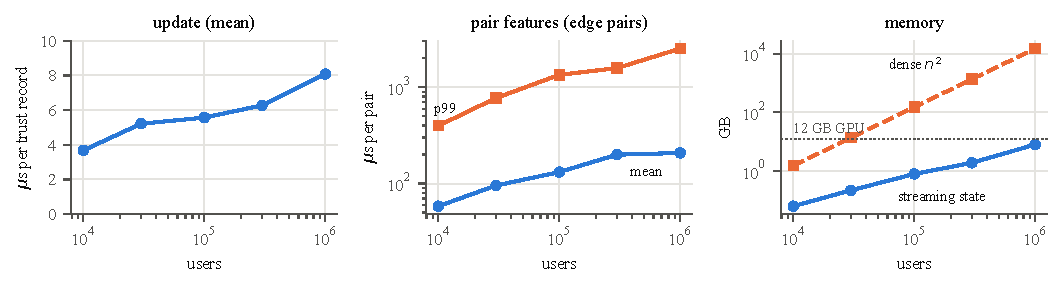
\includegraphics[width=\textwidth]{fig_scale.pdf}
\caption{RQ6: streaming \evi{} state on synthetic temporal graphs with 25 trust records and 25 reviews per user (Python, single thread). Left: mean update time per trust record. Middle: feature time for pairs that become edges (mean and p99). Right: memory of the streaming state vs.\ the $n\times n$ matrices of a dense implementation.}
\label{fig:scale}
\end{figure*}

\subsection{Threats to Validity}
\label{sec:threats}

\emph{Internal.} All methods score identical pairs drawn from fixed seeds, all model selection uses validation data only, and features use only $\mathcal{S}_\tau$. The two \evi{} operating points and their selection rules were pre-registered before their test results were computed. During development we also built a variant that used the 3:1:1 ratio with a different selection rule (maximize validation (b)+(c) among configurations within 0.005 of the best validation AP on (a)). It reached 0.948 / 0.784 / 0.661 on Epinions, i.e., the same robustness as \eviV{} with higher (a). Because its ratio and rule were chosen after inspecting test results, we do not report it as our method, but it shows that the trade-off of RQ3 is not tight. CAT was re-trained with its released code and default hyper-parameters, and our re-trained CAT is 0.003 AP below its reported Epinions number. Guardian, TrustGuard, and TGN use their published default architectures without per-dataset tuning, as does \evi{}. The CAT-H and TGN-H controls reuse one fixed draw of mixed negatives across epochs, whereas CAT's own sampler redraws uniform negatives per batch.
\emph{External.} CiaoDVD lacks trust timestamps, so its result is a static, random-split result, on which classic heuristics are already strong. wiki-RfA has no item categories, which disables CAT's context module, but all methods receive identical inputs. Re-training CAT with much stronger metapath2vec embeddings (20 instead of 5 epochs, 10 walks of length 40 per node) changes its AP by at most $+0.014$ on CiaoDVD and by at most $+0.012$ on wiki-RfA (a) and (c) (three seeds each). It does raise wiki-RfA (b) by 0.056 to 0.470, above both \evi{} variants (0.457, 0.444) but still below TrustGuard (0.523). CAT's results are therefore not an artifact of weak embeddings, except that its wiki-RfA degree-matched score is embedding-sensitive. The wiki-RfA observed subset is small (1{,}182 positives), so we also report all pairs. Scalability beyond $4\times10^4$ users is measured on synthetic graphs, and the real-data stream of the full Ciao release uses random trust times.
\emph{Construct.} Hard negatives can be defined in many ways. We use four generated families, two of which no model is trained on, and real oppose votes where available. The co-review generator falls back to degree-matched negatives for users without reviews (33\% on CiaoDVD). On CiaoDVD, whose trust times are synthetic, active degree-matched negatives nearly coincide with degree-matched ones.

%=====================================================================
\section{Conclusion}
%=====================================================================

The standard trust prediction benchmark rewards popularity. On Epinions a degree product matches the state of the art, and CAT, Guardian, and TrustGuard fall to near chance once candidates are equally popular or equally close. We presented \evi{}, which scores pairs from leakage-safe evidence (directed proximity, activity momentum, and review-order behaviour) kept in an incrementally maintained state and learned with gradient-boosted trees. Against five baselines on Epinions, CiaoDVD, and wiki-RfA, \eviU{} is the best method under the standard protocol on every dataset (Epinions AP 0.970, MRR 0.759). \eviV{}, whose negative mixture is selected on validation data alone, is the most robust on Epinions and CiaoDVD hard negatives ($+0.04$ to $+0.10$ AP over the strongest baseline, $+0.20$ to $+0.31$ over CAT). Re-training CAT and TGN with the same negatives does not close this gap. \evi{} remains accurate for new users (wiki-RfA AUC 0.92--0.94 vs.\ 0.42 for CAT, whose drop is a Simpson's-paradox effect of user history). It absorbs a record in microseconds and scales linearly to a million users. Three results temper these claims. Part of \eviV{}'s margin comes from training on the same negative families it is tested on: holding a generator out costs 0.02--0.08 AP on Epinions and CiaoDVD, and TGN wins on co-review negatives. On wiki-RfA, TrustGuard is best on most hard regimes. No method distinguishes real oppose votes from support votes much beyond chance.

We recommend that trust prediction papers report degree-matched and time-consistent hard negatives, and real distrust where it exists, alongside the uniform protocol. Future work includes larger real platforms, a compiled implementation of the streaming state, and models of opinion \emph{polarity} that use review text, comments, and vote order.

\section*{Artifact Availability}
Code, data conversion scripts, the pre-registration, and per-pair scores for every method and negative regime are available at \url{https://github.com/pshtkdgh9/EviTrust}. Datasets and the CAT code are linked from their original sources.

\bibliographystyle{IEEEtran}
\begin{thebibliography}{99}

\bibitem{tang2015trust}
J.~Tang and H.~Liu, \emph{Trust in Social Media}. Morgan \& Claypool, 2015.

\bibitem{guha2004propagation}
R.~Guha, R.~Kumar, P.~Raghavan, and A.~Tomkins, ``Propagation of trust and distrust,'' in \emph{Proc. WWW}, 2004, pp. 403--412.

\bibitem{yao2013matri}
Y.~Yao, H.~Tong, X.~Yan, F.~Xu, and J.~Lu, ``MATRI: A multi-aspect and transitive trust inference model,'' in \emph{Proc. WWW}, 2013, pp. 1467--1476.

\bibitem{liu2019neuralwalk}
G.~Liu, C.~Li, and Q.~Yang, ``NeuralWalk: Trust assessment in online social networks with neural networks,'' in \emph{Proc. IEEE INFOCOM}, 2019, pp. 1999--2007.

\bibitem{lin2020guardian}
W.~Lin, Z.~Gao, and B.~Li, ``Guardian: Evaluating trust in online social networks with graph convolutional networks,'' in \emph{Proc. IEEE INFOCOM}, 2020, pp. 914--923.

\bibitem{lin2021medley}
W.~Lin and B.~Li, ``Medley: Predicting social trust in time-varying online social networks,'' in \emph{Proc. IEEE INFOCOM}, 2021, pp. 1--10.

\bibitem{wen2023dtrust}
J.~Wen, N.~Jiang, J.~Li, X.~Liu, H.~Chen, Y.~Ren, Z.~Yuan, and Z.~Tu, ``DTrust: Toward dynamic trust levels assessment in time-varying online social networks,'' in \emph{Proc. IEEE INFOCOM}, 2023.

\bibitem{huo2023trustgnn}
C.~Huo, D.~He, C.~Liang, D.~Jin, T.~Qiu, and L.~Wu, ``TrustGNN: Graph neural network-based trust evaluation via learnable propagative and composable nature,'' \emph{IEEE Trans. Neural Netw. Learn. Syst.}, 2023.

\bibitem{jiang2023gatrust}
N.~Jiang, J.~Wen, J.~Li, X.~Liu, and D.~Jin, ``GATrust: A multi-aspect graph attention network model for trust assessment in OSNs,'' \emph{IEEE Trans. Knowl. Data Eng.}, vol.~35, no.~6, pp. 5865--5878, 2023.

\bibitem{wang2024trustguard}
J.~Wang, Z.~Yan, J.~Lan, E.~Bertino, and W.~Pedrycz, ``TrustGuard: GNN-based robust and explainable trust evaluation with dynamicity support,'' \emph{IEEE Trans. Dependable Secure Comput.}, vol.~21, no.~5, pp. 4433--4450, 2024.

\bibitem{wang2025cat}
J.~Wang, Z.~Yan, J.~Lan, X.~Li, and E.~Bertino, ``CAT: Can trust be predicted with context-awareness in dynamic heterogeneous networks?'' \emph{arXiv:2512.11352}, 2025.

\bibitem{usman2025dgten}
M.~Usman and Y.~Lee, ``DGTEN: A robust deep Gaussian based graph neural network for dynamic trust evaluation with uncertainty-quantification support,'' \emph{arXiv:2510.07620}, 2025.

\bibitem{liao2026tchg}
B.~Liao, B.~Deng, Q.~Song, J.~Wang, and J.~Wang, ``TCHG: Tri-trust conditioned heterogeneous graph learning for reliable dynamic trust prediction,'' \emph{arXiv:2606.16611}, 2026.

\bibitem{derr2018sgcn}
T.~Derr, Y.~Ma, and J.~Tang, ``Signed graph convolutional networks,'' in \emph{Proc. IEEE ICDM}, 2018, pp. 929--934.

\bibitem{huang2019sigat}
J.~Huang, H.~Shen, L.~Hou, and X.~Cheng, ``Signed graph attention networks,'' in \emph{Proc. ICANN}, 2019, pp. 566--577.

\bibitem{abdollahpouri2017popularity}
H.~Abdollahpouri, R.~Burke, and B.~Mobasher, ``Controlling popularity bias in learning-to-rank recommendation,'' in \emph{Proc. ACM RecSys}, 2017, pp. 42--46.

\bibitem{wang2019deeptrust}
Q.~Wang, W.~Zhao, J.~Yang, J.~Wu, W.~Hu, and Q.~Xing, ``DeepTrust: A deep user model of homophily effect for trust prediction,'' in \emph{Proc. IEEE ICDM}, 2019, pp. 618--627.

\bibitem{wang2023cdeeptrust}
Q.~Wang, W.~Zhao, J.~Yang, J.~Wu, S.~Xue, and Q.~Xing, ``C-DeepTrust: A context-aware deep trust prediction model in online social networks,'' \emph{IEEE Trans. Neural Netw. Learn. Syst.}, vol.~34, no.~6, pp. 2767--2780, 2023.

\bibitem{wang2023sdeeptrust}
Q.~Wang, W.~Zhao, J.~Yang, and J.~Wu, ``S-DeepTrust: A deep trust prediction method based on sentiment polarity perception,'' \emph{Information Sciences}, vol.~633, pp. 104--121, 2023.

\bibitem{yu2023kgtrust}
Z.~Yu, D.~Jin, C.~Huo, Z.~Wang, X.~Liu, H.~Qi, J.~Wu, and L.~Wu, ``KGTrust: Evaluating trustworthiness of SIoT via knowledge-enhanced graph neural networks,'' in \emph{Proc. ACM Web Conf.}, 2023, pp. 727--736.

\bibitem{xu2023metapath}
Y.~Xu, Z.~Feng, M.~Xing, H.~Wu, S.~Chen, X.~Xue, and S.~Dustdar, ``Metapath-guided multi-headed attention networks for trust prediction in heterogeneous social networks,'' \emph{Knowledge-Based Systems}, vol.~282, p. 111119, 2023.

\bibitem{luo2025gnntrust}
T.~Luo, J.~Wang, Z.~Yan, and E.~Gelenbe, ``Graph neural networks for trust evaluation: Criteria, state-of-the-art, and future directions,'' \emph{IEEE Network}, vol.~39, no.~2, pp. 40--47, 2025.

\bibitem{dong2017metapath2vec}
Y.~Dong, N.~V. Chawla, and A.~Swami, ``metapath2vec: Scalable representation learning for heterogeneous networks,'' in \emph{Proc. ACM KDD}, 2017, pp. 135--144.

\bibitem{libennowell2007link}
D.~Liben-Nowell and J.~Kleinberg, ``The link-prediction problem for social networks,'' \emph{J. Amer. Soc. Inf. Sci. Technol.}, vol.~58, no.~7, pp. 1019--1031, 2007.

\bibitem{adamic2003friends}
L.~A. Adamic and E.~Adar, ``Friends and neighbors on the web,'' \emph{Social Networks}, vol.~25, no.~3, pp. 211--230, 2003.

\bibitem{leskovec2010predicting}
J.~Leskovec, D.~Huttenlocher, and J.~Kleinberg, ``Predicting positive and negative links in online social networks,'' in \emph{Proc. WWW}, 2010, pp. 641--650.

\bibitem{ke2017lightgbm}
G.~Ke, Q.~Meng, T.~Finley, T.~Wang, W.~Chen, W.~Ma, Q.~Ye, and T.-Y. Liu, ``LightGBM: A highly efficient gradient boosting decision tree,'' in \emph{Proc. NeurIPS}, 2017, pp. 3146--3154.

\bibitem{rossi2020tgn}
E.~Rossi, B.~Chamberlain, F.~Frasca, D.~Eynard, F.~Monti, and M.~Bronstein, ``Temporal graph networks for deep learning on dynamic graphs,'' in \emph{ICML Workshop on Graph Representation Learning and Beyond}, 2020.

\bibitem{xu2020tgat}
D.~Xu, C.~Ruan, E.~Korpeoglu, S.~Kumar, and K.~Achan, ``Inductive representation learning on temporal graphs,'' in \emph{Proc. ICLR}, 2020.

\bibitem{sankar2020dysat}
A.~Sankar, Y.~Wu, L.~Gou, W.~Zhang, and H.~Yang, ``DySAT: Deep neural representation learning on dynamic graphs via self-attention networks,'' in \emph{Proc. WSDM}, 2020, pp. 519--527.

\bibitem{wang2021caw}
Y.~Wang, Y.-Y. Chang, Y.~Liu, J.~Leskovec, and P.~Li, ``Inductive representation learning in temporal networks via causal anonymous walks,'' in \emph{Proc. ICLR}, 2021.

\bibitem{yu2023dyglib}
L.~Yu, L.~Sun, B.~Du, and W.~Lv, ``Towards better dynamic graph learning: New architecture and unified library,'' in \emph{Proc. NeurIPS}, 2023.

\bibitem{li2023evaluating}
J.~Li, H.~Shomer, H.~Mao, S.~Zeng, Y.~Ma, N.~Shah, J.~Tang, and D.~Yin, ``Evaluating graph neural networks for link prediction: Current pitfalls and new benchmarking,'' in \emph{Proc. NeurIPS Datasets and Benchmarks}, 2023.

\bibitem{poursafaei2022towards}
F.~Poursafaei, S.~Huang, K.~Pelrine, and R.~Rabbany, ``Towards better evaluation for dynamic link prediction,'' in \emph{Proc. NeurIPS Datasets and Benchmarks}, 2022.

\bibitem{huang2023tgb}
S.~Huang, F.~Poursafaei, J.~Danovitch, M.~Fey, W.~Hu, E.~Rossi, J.~Leskovec, M.~Bronstein, G.~Rabusseau, and R.~Rabbany, ``Temporal graph benchmark for machine learning on temporal graphs,'' in \emph{Proc. NeurIPS Datasets and Benchmarks}, 2023.

\bibitem{guo2014etaf}
G.~Guo, J.~Zhang, D.~Thalmann, and N.~Yorke-Smith, ``ETAF: An extended trust antecedents framework for trust prediction,'' in \emph{Proc. IEEE/ACM ASONAM}, 2014.

\bibitem{west2014exploiting}
R.~West, H.~S. Paskov, J.~Leskovec, and C.~Potts, ``Exploiting social network structure for person-to-person sentiment analysis,'' \emph{Trans. Assoc. Comput. Linguistics}, vol.~2, pp. 297--310, 2014.

\end{thebibliography}

\end{document}
